% !TeX program = xelatex
\documentclass[a4paper,10pt]{article}

% ============================================================================
% សន្លឹកកិច្ចការសិស្សបំពេញចន្លោះ ស-ខ្មៅ និងប្លង់ក្ដារខៀន/ចម្លើយគ្រូ (គ្មាន LCD / គ្មានកន្ត្រៃ)
% មេរៀនទី១ (៨.)៖ ការេ គូប និងឫសការេ ឫសគូប — ត្រូវគ្នា ១០០% នឹង LS_Plan_WN17.tex
% ============================================================================
\usepackage[a4paper, left=1.0cm, right=1.0cm, top=0.75cm, bottom=1.00cm, footskip=0.52cm]{geometry}
\usepackage{amsmath}
\usepackage{unicode-math}
\usepackage{fontspec}
\usepackage{array, colortbl}
\usepackage[table]{xcolor}
\usepackage{enumitem}
\usepackage{pifont}
\usepackage{fancyhdr}
\usepackage{lastpage}
\usepackage{tikz}
\usepackage[most]{tcolorbox}
\usetikzlibrary{calc, arrows.meta, decorations.pathreplacing, positioning, babel}

\makeatletter
\let\@expl@@@mark@update@singlecol@structures@@\relax
\makeatother

\providecommand{\NGSFindFonts}{%
  \IfFileExists{C:/Windows/Fonts/cambria.ttc}{%
    \def\NGSSysPath{C:/Windows/Fonts/}%
    \def\NGSUserPath{C:/Users/KIT/AppData/Local/Microsoft/Windows/Fonts/}%
  }{%
    \IfFileExists{./fonts/KhmerOSsiemreap.ttf}{\def\NGSSysPath{./fonts/}\def\NGSUserPath{./fonts/}}{%
    \IfFileExists{../fonts/KhmerOSsiemreap.ttf}{\def\NGSSysPath{../fonts/}\def\NGSUserPath{../fonts/}}{%
    \IfFileExists{../../fonts/KhmerOSsiemreap.ttf}{\def\NGSSysPath{../../fonts/}\def\NGSUserPath{../../fonts/}}{%
    \IfFileExists{../../../fonts/KhmerOSsiemreap.ttf}{\def\NGSSysPath{../../../fonts/}\def\NGSUserPath{../../../fonts/}}{%
    \IfFileExists{../../../../fonts/KhmerOSsiemreap.ttf}{\def\NGSSysPath{../../../../fonts/}\def\NGSUserPath{../../../../fonts/}}{%
    \IfFileExists{../../../../../fonts/KhmerOSsiemreap.ttf}{\def\NGSSysPath{../../../../../fonts/}\def\NGSUserPath{../../../../../fonts/}}{%
    \IfFileExists{../../../../../../fonts/KhmerOSsiemreap.ttf}{\def\NGSSysPath{../../../../../../fonts/}\def\NGSUserPath{../../../../../../fonts/}}{%
      \def\NGSSysPath{../../../../../../../fonts/}\def\NGSUserPath{../../../../../../../fonts/}%
    }}}}}}}%
  }%
}
\NGSFindFonts

\setmathfont[Path={\NGSSysPath}, FontIndex=1, Scale=1.02]{cambria.ttc}
\defaultfontfeatures{Ligatures=TeX}

\setmainfont[
  Path={\NGSUserPath}, Extension=.ttf, Script=Khmer,
  BoldFont={KhmerOSsiemreap}, BoldFeatures={FakeBold=1.8},
  ItalicFont={KhmerOSsiemreap}, ItalicFeatures={FakeSlant=0.25},
  BoldItalicFont={KhmerOSsiemreap}, BoldItalicFeatures={FakeBold=1.8, FakeSlant=0.25}
]{KhmerOSsiemreap}

\newfontfamily\muol[Path={\NGSUserPath}, Extension=.ttf, Script=Khmer]{KhmerOSmuollight}
\newfontfamily\TimesEn[Path={\NGSSysPath}, Extension=.ttf, BoldFont={timesbd}, ItalicFont={timesi}, BoldItalicFont={timesbi}]{times}
\newfontfamily\CalibriFont[Path={\NGSSysPath}, Extension=.ttf]{calibri}

\XeTeXlinebreaklocale "km"
\XeTeXlinebreakskip = 0pt plus 1pt minus 0.1pt

\definecolor{panelgray}{gray}{0.94}
\definecolor{headgray}{gray}{0.85}

\pagestyle{fancy}
\fancyhf{}
\renewcommand{\headrulewidth}{0pt}
\fancyfoot[L]{\fontsize{7.4pt}{9.5pt}\selectfont អនុវិទ្យាល័យព្រះក្រសាំង \en{|} គ្រូ៖ ហុក ប៊ុនថែន \en{|} មេរៀនទី១ (៨.) ការេ គូប និងឫសការេ ឫសគូប \en{|} ថ្ងៃពុធ ទី១១ ខែវិច្ឆិកា ឆ្នាំ២០២៦}
\fancyfoot[R]{\fontsize{7.8pt}{10pt}\selectfont ទំព័រ \en{\thepage\ / \pageref{LastPage}}}

\setlength{\parindent}{0pt}
\setlength{\parskip}{0pt}
\setlength{\tabcolsep}{4pt}
\newcolumntype{L}[1]{>{\raggedright\arraybackslash}p{#1}}
\newcolumntype{C}[1]{>{\centering\arraybackslash}p{#1}}

\newcommand{\en}[1]{{\TimesEn #1}}
\newcommand{\enbf}[1]{{\TimesEn\bfseries #1}}
\newcommand{\unit}[1]{\,\text{\en{#1}}}
\newcommand{\cnum}[1]{\mbox{\fontsize{10pt}{12pt}\selectfont\ding{\numexpr181+#1\relax}}}
\newcommand{\chkbox}{\tikz[baseline=-0.15ex]\draw[black, line width=0.85pt, fill=white] (0,0) rectangle (0.24cm,0.24cm);}
\newcommand{\ansbox}[1][1.75cm]{\,\tikz[baseline=-0.65ex]\draw[black, line width=0.65pt, fill=white] (0,0) rectangle (#1, 0.42cm);\,}
\newcommand{\dotline}[1][2.2cm]{\makebox[#1]{\dotfill}}

\newcommand{\pagebanner}[2]{%
  \begin{tcolorbox}[
    enhanced, sharp corners, colback=headgray, colframe=black,
    boxrule=1.05pt, boxsep=1pt, top=2.5pt, bottom=2.5pt, left=6pt, right=6pt,
    after skip=3.5pt
  ]
    {\muol\fontsize{9.0pt}{13.2pt}\selectfont #1}\hfill{\fontsize{8.0pt}{11.2pt}\selectfont\textbf{#2}}
  \end{tcolorbox}%
}

\newcommand{\secstrip}[2]{%
  \vspace{3pt}%
  \begin{tcolorbox}[
    enhanced, sharp corners, colback=panelgray, colframe=black,
    boxrule=0.8pt, boxsep=0.8pt, top=2pt, bottom=2pt, left=5pt, right=5pt,
    after skip=3pt
  ]
    {\muol\fontsize{8.5pt}{12.2pt}\selectfont #1}\hfill{\fontsize{7.8pt}{10.8pt}\selectfont\textit{#2}}
  \end{tcolorbox}%
}

\begin{document}
\fontsize{9.5pt}{14.5pt}\selectfont

% ============================================================================
% ទំព័រទី ១៖ សន្លឹកកិច្ចការសិស្ស (ផ្នែកមុខ៖ E1 -> E2 -> E3)
% ============================================================================
\pagebanner{សន្លឹកកិច្ចការសិស្ស \enbf{(}៨\enbf{.} ការេ គូប និងឫសការេ ឫសគូប\enbf{)} \enbf{--} ផ្នែកមុខ}{ថ្នាក់ទី៧ \en{|} សៀវភៅគោល ទំ.១២--១៣}

\begin{tcolorbox}[
  enhanced, sharp corners, colback=white, colframe=black,
  boxrule=0.8pt, boxsep=1.5pt, top=3.5pt, bottom=3.5pt, left=5pt, right=5pt,
  after skip=4pt
]
  \fontsize{9.0pt}{13.0pt}\selectfont
  \textbf{ឈ្មោះសិស្ស៖} \dotline[4.3cm] \quad
  \textbf{សមាជិកក្រុម៖} \dotline[4.3cm] \quad
  \textbf{ថ្នាក់ទី៖} ៧\dotline[0.9cm] \quad
  \textbf{ក្រុមទី៖} \dotline[1.0cm]
\end{tcolorbox}

% --- E1 Engage ---
\secstrip{ផ្នែកទី ១ \enbf{(E1 - Engage)} ៖ បេសកកម្មអន្ទាក់ស្វ័យគុណ $5^2$ និង $5^3$}{រយៈពេល ៣ នាទី (គូស \ding{51} ក្នុង \chkbox)}

\begin{tcolorbox}[
  enhanced, sharp corners, colback=white, colframe=black,
  boxrule=0.8pt, boxsep=2pt, top=4pt, bottom=4pt, left=6pt, right=6pt
]
  គេឱ្យរកផ្ទៃក្រឡាការេជ្រុង $5\unit{cm}$ ($5^2$) និងមាឌគូបទ្រនុង $5\unit{cm}$ ($5^3$) (ឧទាហរណ៍ ៨.១ ទំ.១២)៖\\[3pt]
  $\bullet$ \textbf{តើសិស្សរូបណាគណនាត្រូវ?} \quad
  \chkbox\ \textbf{សិស្ស ក៖} $5^2 = 10\unit{cm}^2, \ 5^3 = 15\unit{cm}^3$ \quad
  \chkbox\ \textbf{សិស្ស ខ៖} $5^2 = 25\unit{cm}^2, \ 5^3 = 125\unit{cm}^3$\\[3pt]
  $\bullet$ \textbf{ហេតុផល៖} ផ្ទៃការេស្មើនឹងជ្រុងគុណនឹង \dotline[1.6cm] ពោលគឺ $5 \times 5 =$ \dotline[1.4cm] $\unit{cm}^2$ ។
\end{tcolorbox}

\vfill

% --- E2 Explore ---
\secstrip{ផ្នែកទី ២ \enbf{(E2 - Explore)} ៖ គំរូធរណីមាត្រការេ-គូប និងឫសការេ-ឫសគូប (ទំ.១២--១៣)}{រយៈពេល ១១ នាទី}

\textbf{សកម្មភាព ១ (\en{E2-A} — ៥ នាទី)៖ ៨.១ ការេនិងគូប (ឧទាហរណ៍ ទំ.១២)}

\begin{tcolorbox}[
  enhanced, sharp corners, colback=white, colframe=black,
  boxrule=0.8pt, boxsep=2.5pt, top=4pt, bottom=4pt, left=6pt, right=6pt
]
  \begin{minipage}{3.8cm}
    \centering
    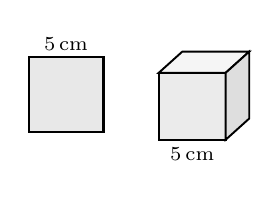
\begin{tikzpicture}[x=1cm, y=1cm, every node/.style={font=\fontsize{7.2pt}{9pt}\selectfont, text=black}]
      \fill[gray!18] (0,0.2) rectangle (0.95,1.15);
      \draw[black, line width=0.8pt] (0,0.2) rectangle (0.95,1.15);
      \node at (0.475,1.32) {$5\unit{cm}$};
      \draw[black, line width=0.8pt, fill=gray!16] (1.65,0.1) rectangle (2.5,0.95);
      \draw[black, line width=0.7pt, fill=gray!8] (1.65,0.95) -- (1.95,1.22) -- (2.8,1.22) -- (2.5,0.95) -- cycle;
      \draw[black, line width=0.7pt, fill=gray!26] (2.5,0.1) -- (2.8,0.37) -- (2.8,1.22) -- (2.5,0.95) -- cycle;
      \node at (2.08,-0.08) {$5\unit{cm}$};
    \end{tikzpicture}
  \end{minipage}\hfill
  \begin{minipage}{14.3cm}
    $\bullet$ \textbf{ផ្ទៃក្រឡាការេ៖} $\underbrace{5 \times 5}_{2\text{ កត្តា}} = 5^2 =$ \ansbox[1.5cm] $\unit{cm}^2$ \quad ($5^2$ អានថា «ប្រាំ\dotline[1.4cm]»)\\[3.5pt]
    $\bullet$ \textbf{មាឌគូប៖} $\underbrace{5 \times 5 \times 5}_{3\text{ កត្តា}} = 5^3 =$ \ansbox[1.6cm] $\unit{cm}^3$ \quad ($5^3$ អានថា «ប្រាំ\dotline[1.4cm]»)
  \end{minipage}
\end{tcolorbox}

\vspace{4pt}
\textbf{សកម្មភាព ២ (\en{E2-B} — ៦ នាទី)៖ ៨.២ ឫសការេនិងឫសគូប សម្គាល់ និងឧទាហរណ៍ ៨.៣ (ទំ.១២--១៣)}

\begin{tcolorbox}[
  enhanced, sharp corners, colback=white, colframe=black,
  boxrule=0.8pt, boxsep=2.5pt, top=4.5pt, bottom=4.5pt, left=6pt, right=6pt
]
  $\bullet$ \textbf{១) ការេមានផ្ទៃក្រឡា $S = 100\unit{cm}^2$៖} ដោយ $100 = 10 \times 10 \implies$ ជ្រុងការេ $a = \sqrt{100} = \sqrt{10^2} =$ \ansbox[1.4cm] $\unit{cm}$\\[3.5pt]
  $\bullet$ \textbf{២) គូបមានមាឌ $V = 27\unit{dm}^3$៖} ដោយ $27 = 3 \times 3 \times 3 \implies$ ទ្រនុងគូប $a = \sqrt[3]{27} = \sqrt[3]{3^3} =$ \ansbox[1.4cm] $\unit{dm}$\\[3.5pt]
  $\bullet$ \textbf{៣) ពាក្យបច្ចេកទេស និងឧទាហរណ៍ ៨.៣ (ទំ.១៣)៖} សញ្ញា $\sqrt{\ }, \sqrt[3]{\ }$ ហៅថា \dotline[1.8cm]; លេខ $100, 27$ ហៅថា \dotline[1.8cm]\\[2.5pt]
  \hspace*{0.3cm}គណនា៖ ក. $\sqrt{625} = \sqrt{25^2} =$ \dotline[1.1cm] \qquad ខ. $9^2 =$ \dotline[1.1cm] \qquad គ. $11^3 = 11\times 11\times 11 =$ \dotline[1.4cm]
\end{tcolorbox}

\vfill

% --- E3 Explain ---
\secstrip{ផ្នែកទី ៣ \enbf{(E3 - Explain)} ៖ រូបមន្តច្រាស និងធនាគារហេតុផល \enbf{B\&W}}{រយៈពេល ៦ នាទី}

\begin{tcolorbox}[
  enhanced, sharp corners, colback=white, colframe=black,
  boxrule=0.85pt, boxsep=2.5pt, top=4pt, bottom=4pt, left=6pt, right=6pt
]
  ចំពោះគ្រប់ចំនួនគត់មិនអវិជ្ជមាន $a \ge 0$៖ \quad
  ១) $a^2 = a \times$ \dotline[0.8cm] $\iff \sqrt{a^2} =$ \dotline[0.8cm] \qquad
  ២) $a^3 = a \times a \times$ \dotline[0.8cm] $\iff \sqrt[3]{a^3} =$ \dotline[0.8cm]\\[3pt]
  ៣) ចំពោះប្រភាគ ($b \ne 0$)៖ $\sqrt[3]{\dfrac{a^3}{b^3}} =$ \dotline[1.1cm] \qquad
  \textbf{ប្រយ័ត្ន៖} ផលបូករ៉ាឌីកាល់ $\sqrt{A} + \sqrt{B} \ne \sqrt{A + B}$ !\\[4pt]
  \tikz\draw[black, dashed, line width=0.5pt] (0,0) -- (18.4cm,0);\\[3.5pt]
  \fontsize{8.8pt}{13.0pt}\selectfont
  \textbf{ធនាគារហេតុផល (\en{Warrant Bank})៖} \quad
  \cnum{1} \textbf{ការេ/គូប៖} $a^2 = a\times a$ ($\ne 2a$); $a^3 = a\times a\times a$ ($\ne 3a$) \quad
  \cnum{2} \textbf{ឫសការេ៖} $\sqrt{a^2} = a$ ($a\ge 0$)\\
  \cnum{3} \textbf{ឫសគូប៖} $\sqrt[3]{a^3} = a$ និង $\sqrt[3]{a^3/b^3} = a/b$ \quad
  \cnum{4} \textbf{កន្សោមរ៉ាឌីកាល់៖} បញ្ចេញពីរ៉ាឌីកាល់ម្ដងមួយតួមុនបូក/ដក/គុណ
\end{tcolorbox}

% ============================================================================
% ទំព័រទី ២៖ សន្លឹកកិច្ចការសិស្ស (ផ្នែកខាងខ្នង៖ E4 -> E5 -> កិច្ចការផ្ទះ)
% ============================================================================
\clearpage
\pagebanner{សន្លឹកកិច្ចការសិស្ស \enbf{(}៨\enbf{.} ការេ គូប និងឫសការេ ឫសគូប\enbf{)} \enbf{--} ផ្នែកខាងខ្នង}{ថ្នាក់ទី៧ \en{|} សៀវភៅគោល ទំ.១៣--១៤}

% --- E4 Elaborate ---
\secstrip{ផ្នែកទី ៤ \enbf{(E4 - Elaborate)} ៖ លំហាត់គំរូ ក និង ខ (សៀវភៅគោល ទំ.១៣)}{រយៈពេល ១០ នាទី}

\begin{tcolorbox}[
  enhanced, sharp corners, colback=white, colframe=black,
  boxrule=0.8pt, boxsep=2.5pt, top=4.5pt, bottom=4.5pt, left=6pt, right=6pt
]
  $\bullet$ \textbf{១) លំហាត់គំរូ ក (ទំ.១៣)៖} គណនា $\sqrt{4\,900} + \sqrt{1\,600}$\\[3pt]
  \hspace*{0.3cm}$= \sqrt{(\dotline[1.0cm])^2} + \sqrt{(\dotline[1.0cm])^2} =$ \dotline[1.1cm] $+$ \dotline[1.1cm] $=$ \ansbox[1.6cm] (\cnum{2}, \cnum{4})\\[4pt]
  $\bullet$ \textbf{២) លំហាត់គំរូ ខ (ទំ.១៣)៖} គណនា $\sqrt[3]{\dfrac{8}{125}} = \sqrt[3]{\dfrac{2}{5} \times \dfrac{2}{5} \times \dfrac{2}{5}} = \sqrt[3]{\left(\dfrac{\dotline[0.8cm]}{\dotline[0.8cm]}\right)^3} =$ \ansbox[1.6cm] (\cnum{3})\\[3.5pt]
  \fontsize{8.8pt}{12.8pt}\selectfont
  \textbf{ឆ្លុះបញ្ចាំង (\en{EIA Looking-Back})៖} ហេតុអ្វីមិនអាចបូកជា $\sqrt{4\,900 + 1\,600} = \sqrt{6\,500}$? ព្រោះ $110^2 =$ \dotline[1.6cm] $\ne 6\,500$ !
\end{tcolorbox}

\vfill

% --- E5 Evaluate ---
\secstrip{ផ្នែកទី ៥ \enbf{(E5 - Evaluate)} ៖ លំហាត់ប្រតិបត្តិ (ទំ.១៣) សំណួរវិនិច្ឆ័យ \enbf{A--D} និងសំបុត្រចេញ}{រយៈពេល ១០ នាទី}

\begin{tcolorbox}[
  enhanced, sharp corners, colback=white, colframe=black,
  boxrule=0.8pt, boxsep=2.5pt, top=4.5pt, bottom=4.5pt, left=6pt, right=6pt
]
  \textbf{១) ប្រតិបត្តិជាក្រុមតូច ៣ នាក់ (សៀវភៅគោល ទំ.១៣)៖}\\[3.5pt]
  $\bullet$ \textbf{ក.} គណនា $\sqrt{12^2} \times \sqrt{34^2} =$ \dotline[1.2cm] $\times$ \dotline[1.2cm] $=$ \ansbox[1.8cm] (\cnum{2})\\[3.5pt]
  $\bullet$ \textbf{ខ.} គណនា $\sqrt[3]{\dfrac{216}{1\,000}} = \sqrt[3]{\left(\dfrac{\dotline[0.9cm]}{10}\right)^3} = \dfrac{\dotline[0.9cm]}{10} =$ \ansbox[1.6cm] (\emph{សម្រួលប្រភាគជាទម្រង់បង្រួម — \cnum{3}})\\[4pt]
  \textbf{២) បិទបេសកកម្ម \en{E1}៖} សិស្ស \dotline[1.0cm] ត្រឹមត្រូវ ព្រោះ $5^2 =$ \dotline[1.1cm] $\unit{cm}^2$ និង $5^3 =$ \dotline[1.3cm] $\unit{cm}^3$ (\cnum{1}) ។
\end{tcolorbox}

\vspace{4pt}

\begin{tcolorbox}[
  enhanced, sharp corners, colback=white, colframe=black,
  boxrule=0.8pt, boxsep=2.5pt, top=4.5pt, bottom=4.5pt, left=6pt, right=6pt
]
  \textbf{៣) សំណួរវិនិច្ឆ័យ \en{A--D} (តើតម្លៃនៃកន្សោម $4^3 - \sqrt{36}$ ស្មើនឹងប៉ុន្មាន? — គូសរង្វង់ រួចលើកម្រាមដៃ ១--៤)៖}\\[3.5pt]
  \textbf{\en{A.}} $6$ \qquad\qquad
  \textbf{\en{B.}} $46$ \qquad\qquad
  \textbf{\en{C.}} $58$ \qquad\qquad
  \textbf{\en{D.}} $28$\\[4.5pt]
  \tikz\draw[black, dashed, line width=0.5pt] (0,0) -- (18.4cm,0);\\[3.5pt]
  \textbf{៤) សំបុត្រចេញ ៦០ វិនាទី៖} គណនា $3^3 + \sqrt[3]{64} =$ \dotline[1.2cm] $+$ \dotline[1.1cm] $=$ \ansbox[1.8cm] ។
\end{tcolorbox}

\vfill

% --- Homework ---
\begin{tcolorbox}[
  enhanced, sharp corners, colback=panelgray, colframe=black,
  boxrule=0.95pt, boxsep=2.5pt, top=4pt, bottom=4pt, left=6pt, right=6pt
]
  {\muol\fontsize{9.0pt}{13.0pt}\selectfont កិច្ចការផ្ទះបញ្ចប់មេរៀនទី១ \enbf{(}សៀវភៅគោល ទំ.១៤ លេខ ៨ និង លេខ ៩\enbf{)}}\\[3pt]
  \fontsize{8.8pt}{12.8pt}\selectfont
  $\bullet$ \textbf{លេខ ៨ (គណនាតម្លៃ)៖} \quad ក. $2^2 \times 5^3$ \qquad ខ. $5^3 + 3^2$ \qquad គ. $8^2 - 3^3$ \qquad ឃ. $3x^2$ បើ $x = 5$ ។\\[2pt]
  $\bullet$ \textbf{លេខ ៩ (សម្រួល)៖} \quad ក. $\sqrt{9}\times\sqrt{16}$ \qquad ខ. $4^2 - \sqrt{4}$ \qquad គ. $\sqrt{100}\times\sqrt{196}$ \qquad ឃ. $\dfrac{5^3 + \sqrt[3]{64} - \sqrt[3]{8}}{3^3}$ ។
\end{tcolorbox}

% ============================================================================
% ទំព័រទី ៣៖ ទំព័រគ្រូបង្រៀន (គំរូប្លង់ក្ដារខៀន ៣ ផ្នែក + ចម្លើយផ្ទៀងផ្ទាត់រហ័ស)
% ============================================================================
\clearpage
\pagebanner{ទំព័រគ្រូបង្រៀន ៖ ប្លង់ក្ដារខៀន \enbf{(}គ្មាន \enbf{LCD)} និងចម្លើយផ្ទៀងផ្ទាត់រហ័ស}{៨. ការេ គូប និងឫសការេ ឫសគូប (\en{WN17})}

\secstrip{១. គំរូប្លង់បែងចែកក្ដារខៀន ៣ ផ្នែក សម្រាប់ថ្នាក់រៀនគ្មាន \enbf{LCD}}{សម្រាប់គ្រូប្រើដីស/ហ្វឺត}

\begin{center}
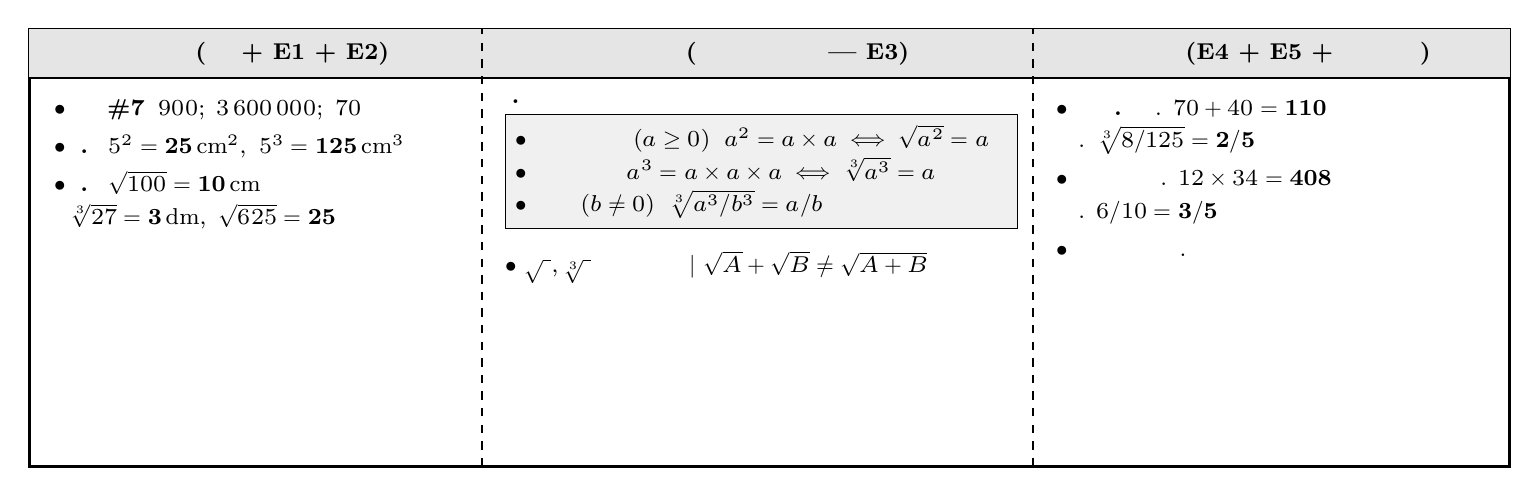
\begin{tikzpicture}[x=1cm, y=1cm, every node/.style={font=\fontsize{8.3pt}{11.8pt}\selectfont, text=black}]
  \draw[black, line width=1.1pt] (0,0) rectangle (18.8,5.55);
  \fill[gray!20] (0,4.93) rectangle (18.8,5.55);
  \draw[black, line width=0.7pt] (0,4.93) -- (18.8,4.93);
  \draw[black, dashed, line width=0.7pt] (5.75,0) -- (5.75,5.55);
  \draw[black, dashed, line width=0.7pt] (12.75,0) -- (12.75,5.55);

  \node at (2.875,5.24) {\textbf{ផ្នែកឆ្វេង (កំណែ + \en{E1} + \en{E2})}};
  \node at (9.25,5.24) {\textbf{ផ្នែកកណ្ដាល (ខ្លឹមសារគោលរក្សាទុក — \en{E3})}};
  \node at (15.775,5.24) {\textbf{ផ្នែកស្ដាំ (\en{E4} + \en{E5} + កិច្ចការផ្ទះ)}};

  % Left
  \node[anchor=north west, text width=5.30cm] at (0.20,4.78) {%
    $\bullet$ \textbf{កំណែ \#7៖} $900;\ 3\,600\,000;\ 70$\\[2pt]
    $\bullet$ \textbf{៨.១៖} $5^2 = \mathbf{25}\unit{cm}^2,\ 5^3 = \mathbf{125}\unit{cm}^3$\\[2pt]
    $\bullet$ \textbf{៨.២៖} $\sqrt{100} = \mathbf{10}\unit{cm}$\\
    \hspace*{0.2cm}$\sqrt[3]{27} = \mathbf{3}\unit{dm},\ \sqrt{625} = \mathbf{25}$
  };

  % Center
  \node[anchor=north west, text width=6.65cm] at (5.92,4.78) {%
    {\muol\fontsize{8.4pt}{12pt}\selectfont ៨\enbf{.} ការេ គូប និងឫសការេ ឫសគូប}\\[3pt]
    \tikz\node[draw=black, fill=gray!12, inner sep=3.5pt, text width=6.25cm]{%
      $\bullet$ ការេ និងឫសការេ ($a\ge 0$)៖ $a^2 = a\times a \iff \sqrt{a^2} = a$\\
      $\bullet$ គូប និងឫសគូប៖ $a^3 = a\times a\times a \iff \sqrt[3]{a^3} = a$\\
      $\bullet$ ប្រភាគ ($b\ne 0$)៖ $\sqrt[3]{a^3 / b^3} = a / b$
    };\\[4pt]
    $\bullet$ $\sqrt{\ }, \sqrt[3]{\ }$ ហៅថារ៉ាឌីកាល់ $\mid$ $\sqrt{A}+\sqrt{B} \ne \sqrt{A+B}$
  };

  % Right
  \node[anchor=north west, text width=5.65cm] at (12.92,4.78) {%
    $\bullet$ \textbf{គំរូទំ.១៣៖} ក. $70+40=\mathbf{110}$\\
    \hspace*{0.2cm}ខ. $\sqrt[3]{8/125} = \mathbf{2/5}$\\[2pt]
    $\bullet$ \textbf{ប្រតិបត្តិ៖} ក. $12\times 34 = \mathbf{408}$\\
    \hspace*{0.2cm}ខ. $6/10 = \mathbf{3/5}$\\[2pt]
    $\bullet$ \textbf{កិច្ចការផ្ទះ៖} ទំ.១៤ លេខ ៨ និង លេខ ៩
  };
\end{tikzpicture}
\end{center}

\vfill
\secstrip{២. ចម្លើយផ្ទៀងផ្ទាត់រហ័សសម្រាប់សន្លឹកកិច្ចការសិស្ស \enbf{(}ទំព័រ ១ និង ទំព័រ ២\enbf{)}}{\en{Answer Key}}

\begin{tcolorbox}[
  enhanced, sharp corners, colback=white, colframe=black,
  boxrule=0.8pt, boxsep=2.5pt, top=4.5pt, bottom=4.5pt, left=6pt, right=6pt
]
  \fontsize{8.9pt}{13.2pt}\selectfont
  $\bullet$ \textbf{ផ្នែក \en{E1}៖} \textbf{សិស្ស ខ} ត្រឹមត្រូវ ($25\unit{cm}^2$ និង $125\unit{cm}^3$) ព្រោះផ្ទៃការេស្មើនឹងជ្រុងគុណនឹង\textbf{ជ្រុង} ($5\times 5 = 25$) ។\\[2pt]
  $\bullet$ \textbf{ផ្នែក \en{E2}៖} \textbf{សកម្មភាព ១៖} $25\unit{cm}^2$ (ប្រាំការេ); $125\unit{cm}^3$ (ប្រាំគូប) ។ \textbf{សកម្មភាព ២៖} $10\unit{cm}$; $3\unit{dm}$; រ៉ាឌីកាល់ និង រ៉ាឌីកង់; $25,\ 81,\ 1\,331$ ។\\[2pt]
  $\bullet$ \textbf{ផ្នែក \en{E4}៖} គំរូ ក $= \sqrt{70^2} + \sqrt{40^2} = 70 + 40 = \mathbf{110}$; គំរូ ខ $= \sqrt[3]{(2/5)^3} = \mathbf{2/5}$ ។ \en{EIA}៖ $110^2 = 12\,100 \ne 6\,500$ ។\\[2pt]
  $\bullet$ \textbf{ផ្នែក \en{E5}៖} \textbf{១) ប្រតិបត្តិទំ.១៣៖} ក. $12\times 34 = \mathbf{408}$; ខ. $6/10 = \mathbf{3/5}$ ។ \textbf{២) បិទ \en{E1}៖} សិស្ស ខ ($25;\ 125$) ។ \textbf{៣) វិនិច្ឆ័យ \en{A--D}៖} \textbf{ជម្រើស \en{C}} ($64-6=58$) ។ \textbf{៤) សំបុត្រចេញ៖} $27 + 4 = \mathbf{31}$ ។
\end{tcolorbox}

\vfill
\secstrip{៣. ចម្លើយលម្អិតនៃកិច្ចការផ្ទះបញ្ចប់មេរៀនទី១ \enbf{(}សៀវភៅគោល ទំ.១៤ លេខ ៨ និង លេខ ៩\enbf{)}}{សៀវភៅគោល ទំ.១៤}

\begin{tcolorbox}[
  enhanced, sharp corners, colback=white, colframe=black,
  boxrule=0.8pt, boxsep=2.5pt, top=4.5pt, bottom=4.5pt, left=6pt, right=6pt
]
  \fontsize{8.7pt}{12.9pt}\selectfont
  $\bullet$ \textbf{លេខ ៨៖} ក. $2^2\times 5^3 = 4\times 125 = \mathbf{500}$ $\mid$ ខ. $5^3+3^2 = 125+9 = \mathbf{134}$ $\mid$ គ. $8^2-3^3 = 64-27 = \mathbf{37}$ $\mid$ ឃ. $3x^2 = 3\times 5^2 = 3\times 25 = \mathbf{75}$ ។\\[2pt]
  $\bullet$ \textbf{លេខ ៩៖} ក. $\sqrt{9}\times\sqrt{16} = 3\times 4 = \mathbf{12}$ $\mid$ ខ. $4^2-\sqrt{4} = 16-2 = \mathbf{14}$ $\mid$ គ. $\sqrt{100}\times\sqrt{196} = 10\times 14 = \mathbf{140}$ $\mid$ ឃ. $\dfrac{125 + 4 - 2}{27} = \mathbf{\dfrac{127}{27}}$ ។
\end{tcolorbox}

\vfill
\secstrip{៤. ចំណុចប្រុងប្រយ័ត្នគរុកោសល្យសម្រាប់គ្រូ \enbf{(}ការយល់ច្រឡំសំខាន់ៗរបស់សិស្ស\enbf{)}}{\en{Pedagogical Watchlist}}

\begin{tcolorbox}[
  enhanced, sharp corners, colback=panelgray, colframe=black,
  boxrule=0.85pt, boxsep=2.5pt, top=4.5pt, bottom=4.5pt, left=6pt, right=6pt
]
  \fontsize{8.7pt}{12.9pt}\selectfont
  $\bullet$ \textbf{អន្ទាក់ក្នុងលំហាត់ទំ.១៤ លេខ ៨ ឃ ($3x^2$ បើ $x=5$)៖} ត្រូវណែនាំសិស្សឱ្យលើក $x$ ជាការេជាមុនសិន ($3\times 5^2 = 3\times 25 = 75$) កុំឱ្យច្រឡំគុណ $(3\times 5)^2 = 15^2 = 225$!\\[2pt]
  $\bullet$ \textbf{ការរក $\sqrt{196}$ ក្នុងលេខ ៩ គ ដោយគ្មានម៉ាស៊ីនគិតលេខ៖} ណែនាំឱ្យសិស្សសង្កេត $10^2 = 100$ និង $15^2 = 225$ ហើយខ្ទង់រាយបញ្ចប់ដោយលេខ $6$ ($\to 14^2 = 196$) ។
\end{tcolorbox}

\end{document}
